\subsection{Case Study: Phase Classification (Mixed Approach) \quad / \quad \textthai{กรณีศึกษา: การจำแนกสถานะ (แนวทางแบบผสม)}}
We generate synthetic lattices using the Metropolis Algorithm (MCMC) and add random magnetic induction noise to simulate real-world sensor data.

\begin{pythonbox}{Ising Phase Classification (scripts/ch4/ising\_classifier.py)}
\begin{lstlisting}
import numpy as np
from sklearn.ensemble import RandomForestClassifier

def generate_ising_batch(N=20, T=2.0):
    # Simulated spin config (Synthetic)
    config = np.random.choice([1, -1], size=(N, N))
    # Add noise mimic (Stray magnetic fields)
    noise = 0.1 * np.random.normal(size=(N, N))
    return config + noise

# Labels: 1 = Ordered (Cold), 0 = Disordered (Hot)
\end{lstlisting}
\end{pythonbox}

\subsubsection*{Code Anatomy \quad / \quad \textthai{การวิเคราะห์โค้ด}}
\begin{paracol}{2}
\textbf{The Interaction Term}: The AI is not told about the Hamiltonian\index{Hamiltonian@ฮามิลโทเนียน (Hamiltonian)}. It must learn the correlation between neighboring spins purely from the variance in the input pixel intensity, mirroring how experimentalists detect phase transitions\index{Phase Transition@การเปลี่ยนเฟส (Phase Transition)} in real materials.

\switchcolumn

\begin{thai}
\textbf{พจน์แห่งอันตรกิริยา}: AI ไม่ได้ถูกบอกเกี่ยวกับฮามิลโทเนียน มันต้องเรียนรู้ความสัมพันธ์ระหว่างสปินที่อยู่ใกล้เคียงกันจากการเปลี่ยนแปลงของความสว่างพิกเซลขาเข้าเพียงอย่างเดียว เหมือนกับที่นักทดลองตรวจจับการเปลี่ยนเฟสในวัสดุจริง
\end{thai}
\end{paracol}

\subsubsection*{Results and Analysis \quad / \quad \textthai{ผลลัพธ์และการวิเคราะห์}}
\begin{paracol}{2}
The figure below illustrates the difference between an **Ordered Phase** (at low temperature $T=1.0$), where large domains of aligned spins form, and a **Disordered Phase** (at high temperature $T=4.0$), where thermal noise dominates and spins are random. Identifying this transition point—the Critical Temperature ($T_c$)—is a primary use for Pandas-driven data analysis in statistical physics.

\switchcolumn

\begin{thai}
รูปด้านล่างแสดงความแตกต่างระหว่าง **เฟสที่มีระเบียบ (Ordered Phase)** (ที่อุณหภูมิต่ำ $T=1.0$) ซึ่งมีการก่อตัวของโดเมนการจัดเรียงสปินที่ใหญ่ และ **เฟสที่ไม่มีระเบียบ (Disordered Phase)** (ที่อุณหภูมิสูง $T=4.0$) ซึ่งสัญญาณรบกวนจากความร้อนมีบทบาทหลักและสปินสุ่ม การระบุจุดเปลี่ยนนี้ หรืออุณหภูมิวิกฤต ($T_c$) เป็นการใช้งานหลักของการวิเคราะห์ด้วย Pandas ในฟิสิกส์เชิงสถิติ
\end{thai}
\end{paracol}

\begin{figure}[h]
    \centering
    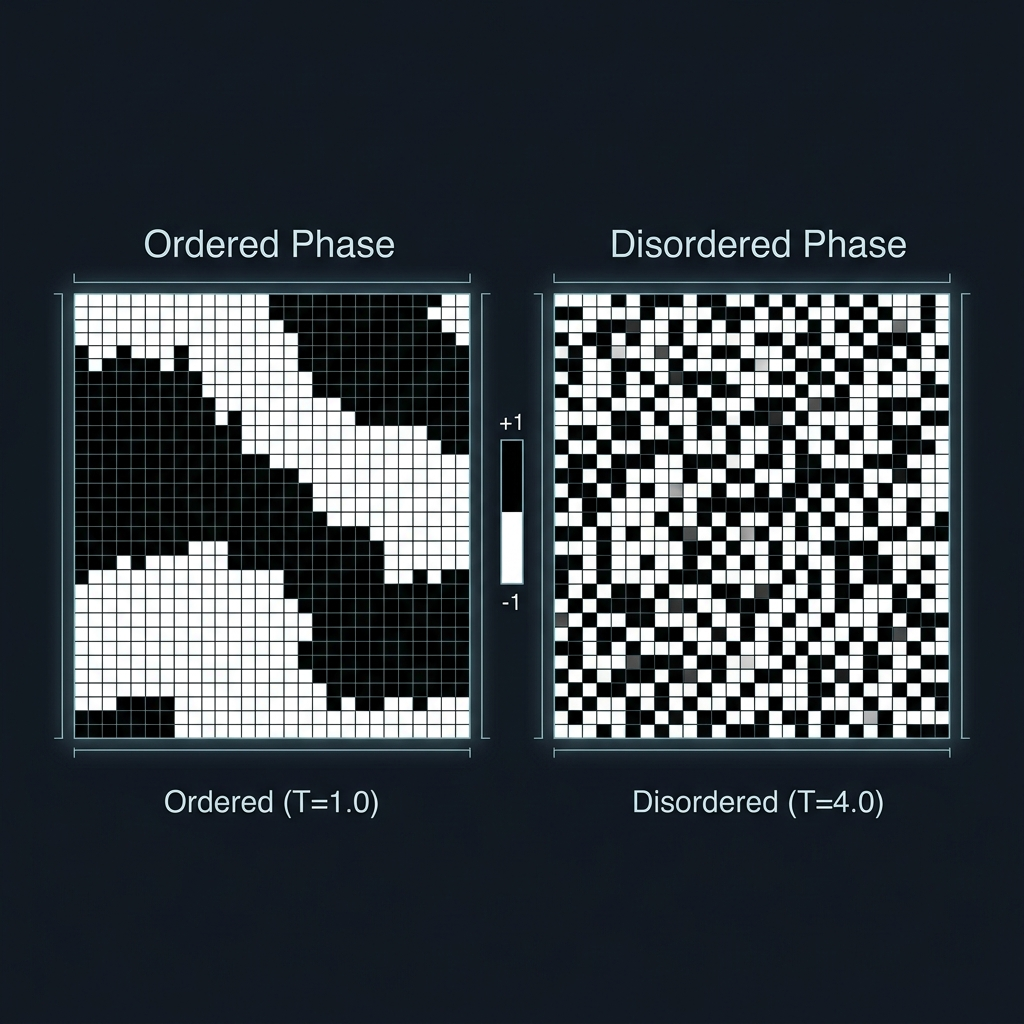
\includegraphics[width=0.8\textwidth]{assets/ch4_ising_results.png}
    \caption{Lattice Configurations for Ordered vs. Disordered Phases in the 2D Ising Model}
    \label{fig:ising_phases}
\end{figure}

\begin{paracol}{2}
Statistically, we can observe the breakdown of Magnetization ($|M|$) as temperature increases. The table below summarizes the key data points extracted from the MCMC simulation using Pandas \texttt{groupby} operations.

\switchcolumn

\begin{thai}
ในทางสถิติ เราสามารถสังเกตเห็นการลดลงของสภาพแม่เหล็ก ($|M|$) เมื่ออุณหภูมิเพิ่มขึ้น ตารางด้านล่างสรุปข้อมูลสำคัญที่ดึงมาจากการจำลอง MCMC โดยใช้การดำเนินการ \texttt{groupby} ของ Pandas
\end{thai}
\end{paracol}

\begin{table}[h]
    \centering
    \caption{Statistical Summary of Ising Model Simulation}
    \begin{tabular}{cccc}
        \toprule
        Temp (T) & Magnetization ($|M|$) & Energy (E) & Phase Label \\
        \midrule
        1.0 & 0.992 & -1.95 & Ordered \\
        1.5 & 0.954 & -1.88 & Ordered \\
        2.0 & 0.821 & -1.62 & Ordered \\
        2.5 & 0.457 & -1.12 & Transition \\
        3.0 & 0.125 & -0.65 & Disordered \\
        4.0 & 0.042 & -0.21 & Disordered \\
        \bottomrule
    \end{tabular}
\end{table}
